\documentclass{article}

% Das babel Paket passt Zeichen und Überschriften nach Deutsch (Schweiz) Standards an.
\usepackage[nswissgerman]{babel}

% Das graphicx Paket ermöglicht das Einfügen von Bildern. PDFs können auch eingefügt werden.
\usepackage{graphicx}
\graphicspath{{./assets/images/}}
% Diese Einstellung wird benötigt um PDFs der Version 1.7 einfügen zu können.
\pdfminorversion=7

% Das hyperref Paket erstellt automatisch Hyperlinks auf allen Referenzen.
\usepackage{hyperref}
\hypersetup{colorlinks,citecolor=black,filecolor=black,linkcolor=black,urlcolor=black}

% Das glossaries Paket ermöglicht das Erfassen von Wörtern und Acronymen. Es kann auch automatisch ein Glossar erstellt werden.
\usepackage[acronym]{glossaries}
\makenoidxglossaries
\newglossaryentry{BIOS}{name=BIOS,description={Firmware zur grundlegenden Steuerung von Computer-Hardware}}
\newacronym{CI/CD}{CI/CD}{Corporate Identity / Corporate Design}

% Das biblatex Paket ermöglicht das Referenzieren auf eine Biblographie.
\usepackage[style=numeric]{biblatex}
\addbibresource{./assets/bibliographies/references.bib}
\DeclareBibliographyAlias{video}{misc}

% Diese Befehle werden benötigt um die Überschriften des Abbildungs- und Tabellenverzeichnis im Inhaltsverzeichnis anzeigen zu lassen.
\makeatletter\renewcommand\listoffigures{\subsection{\listfigurename}\@mkboth{\MakeUppercase\listfigurename}{\MakeUppercase\listfigurename}\@starttoc{lof}}\makeatother
\makeatletter\renewcommand\listoftables{\subsection{\listtablename}\@mkboth{\MakeUppercase\listtablename}{\MakeUppercase\listtablename}\@starttoc{lot}}\makeatother

% Das csquotes Paket liefert Befehle zur Formatierung von Zitaten.
\usepackage{csquotes}

% Das placeins Paket liefert Befehle zur Platzierung von Abbildungen und Tabellen.
\usepackage[section]{placeins}

% Das fancyhdr Paket liefter Befehle zur Formatierung der Kopf- und Fusszeile.
\usepackage{fancyhdr}
\usepackage{lastpage}
\pagestyle{fancy}
\fancyhf{}
\lhead{Vorlage für wissenschaftliche Dokumente mit \LaTeX}
\rhead{Nicholas Weidmann}
\rfoot{Seite \thepage\ von \pageref{LastPage}}

\title{Vorlage für wissenschaftliche Dokumente \protect\\ mit \LaTeX\\
\bigskip\large Höhere Fachschule Uster}
\author{Nicholas Weidmann}
\date{August 2022}

% Konfiguriert hyperref um den Titel und Autor in den PDF Metadaten zu setzen.
\hypersetup{pdftitle={Vorlage für wissenschaftliche Dokumente mit LaTeX},pdfauthor={Nicholas Weimdann}}

\begin{document}

\begin{titlepage}
  \maketitle
  \thispagestyle{empty}
\end{titlepage}

\tableofcontents
\clearpage

\section{Auflistung und Wörter und Akronyme}
\begin{itemize}
  \item \gls{BIOS} im Stil des \acrshort{CI/CD}
  \item \acrfull{CI/CD}
\end{itemize}

\subsection{Blockzitat}
\paragraph{Paragraf} Das Blockzitat.

\begin{displayquote}
  TeX ([t$\varepsilon$x], im deutschsprachigen Raum auch [t$\varepsilon$ç]), in Eigenschreibweise \TeX, ist ein von Donald E. Knuth ab 1977 entwickeltes und 1986 fertiggestelltes Textsatzsystem mit eingebauter Makrosprache (die ebenfalls TeX genannt wird).
  \cite{noauthor_tex_2022}
  \label{qte:tex}
\end{displayquote}

\noindent Text ohne Einrückung.

\subsubsection{Tabellen und Grafiken}

\begin{figure}[ht!]
  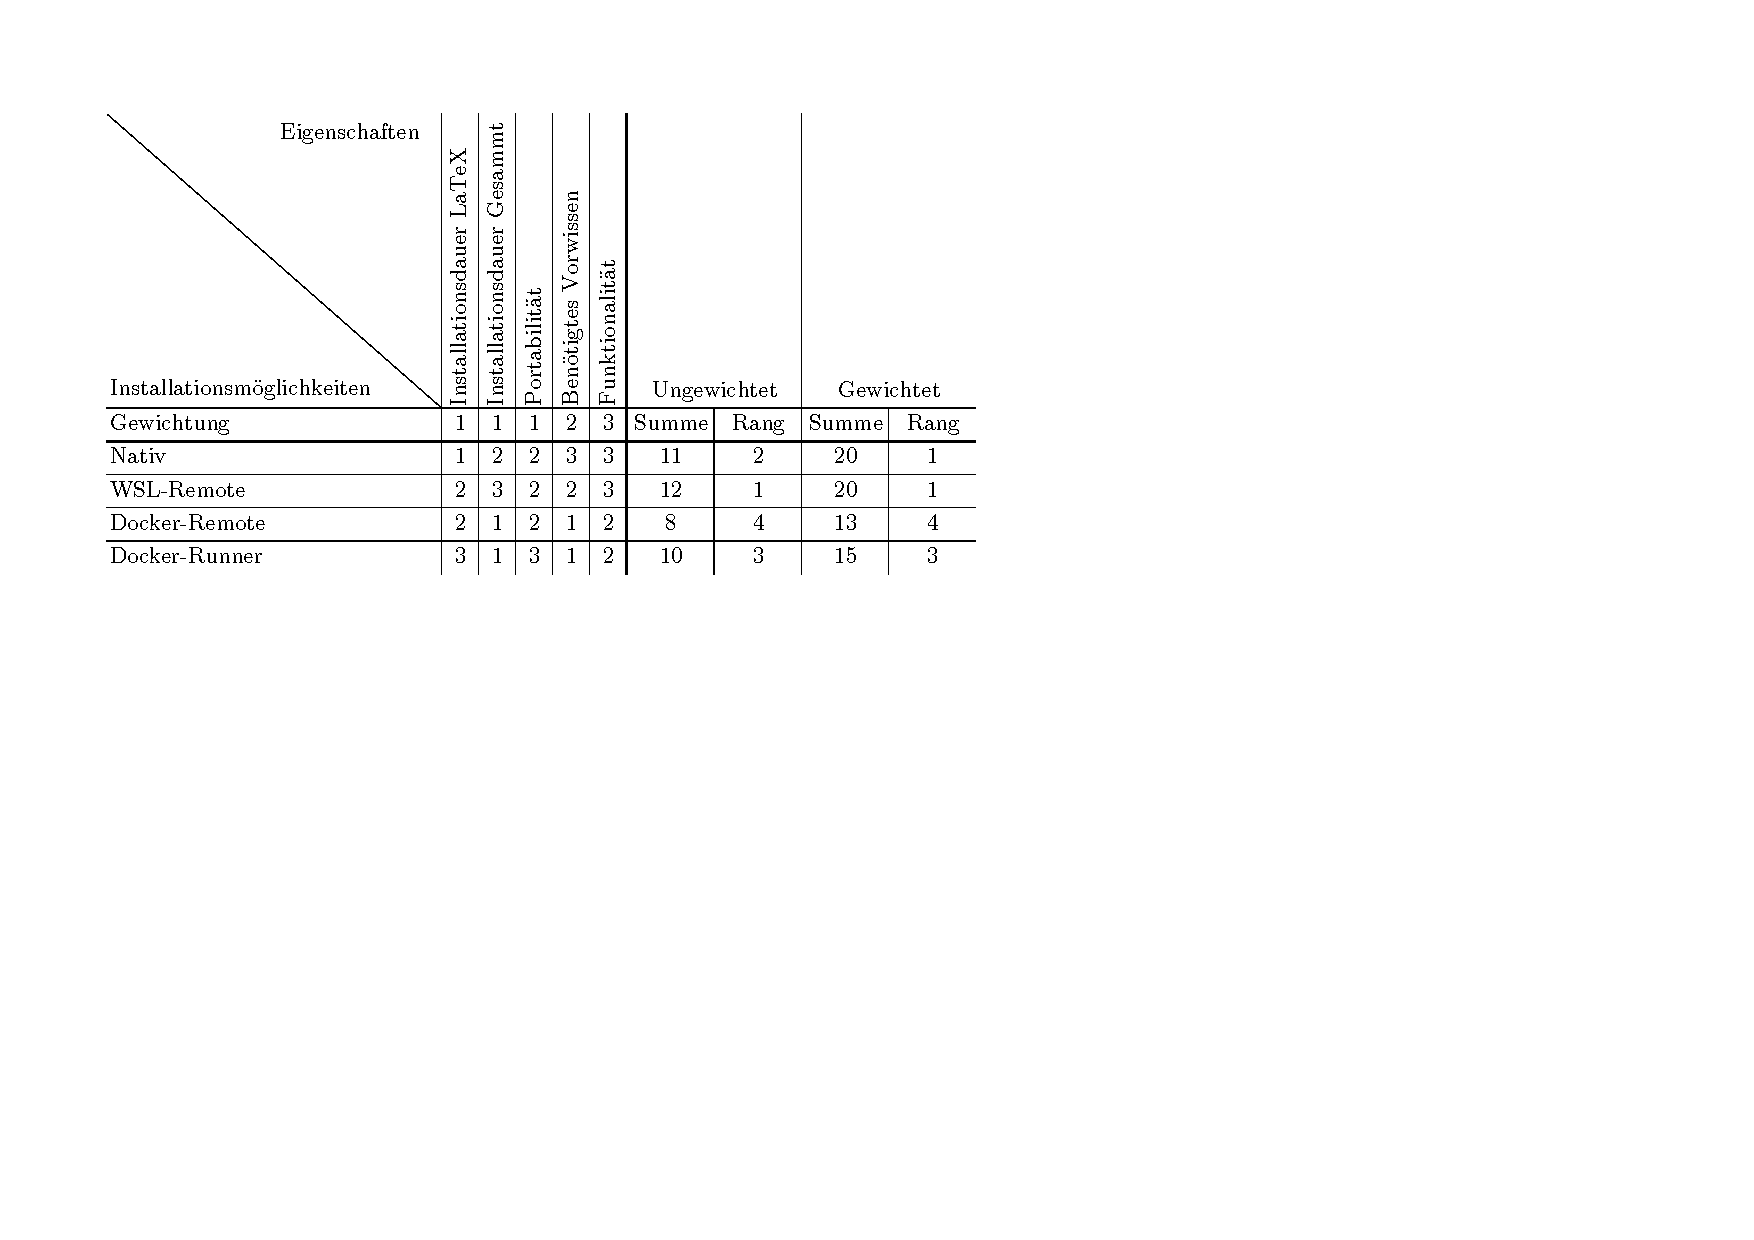
\includegraphics[width=\textwidth]{installoptions_grading.pdf}
  \caption{Installationsmöglichkeiten Bewertung (eigene Darstellung inspiriert von Technische Universität Braunschweig)\cite{noauthor_gewichtete_nodate}}
  \label{fig:installoptions_grading}
\end{figure}

\begin{table}
  \centering
  \begin{tabular}{p{0.12\linewidth}|p{0.8\linewidth}}
    ID       & Kriterium                           \\
    \hline
    Krit-001 & \textbf{Kriterium 1.} Beschreibung. \\
    \hline
    Krit-002 & \textbf{Kriterium 2.} Beschreibung. \\
    \hline
    Krit-003 & \textbf{Kriterium 3.} Beschreibung. \\
  \end{tabular}
  \caption{Kriterien}
  \label{tbl:krit}
\end{table}

\clearpage
\section{Referenzen}
\subsection{Glossar}
\printnoidxglossary[title=\large Wörter]
\printnoidxglossary[type=\acronymtype,title=\large Akronyme]

\subsection{Quellen}
\printbibliography[heading=none]

\listoffigures

\listoftables

\section{Anhang}

\end{document}
